\chapter{约束下的子集选择}
\label{chap:constrained-subset-selection}

上一章的传感器实例里，四个传感器合起来能覆盖全部$16$格。实际中名额或经费有限：只能装两个传感器时该装哪两个？各传感器价格不同、总经费固定时又该怎样选？这类问题在有限底集上最大化一个集合函数，同时限制所选子集的规模或总成本。小实例可以枚举全部可行子集，底集稍大时枚举就不可行，于是需要只看少量子集、又能说明结果离最优有多远的方法。

本章研究逐轮加入元素的贪心规则，分基数约束和预算约束两节。第~\ref{sec:graph-cardinality-selection}节在“至多选$k$个”的限制下每轮加入边际增益最大的元素，证明目标归一化、单调且次模时，所得值不低于最优值的$1-(1-1/k)^k$倍；同一节还说明次模性怎样让旧增益成为当前增益的上界，从而得到减少求值次数的惰性贪心。第~\ref{sec:graph-budget-selection}节让各元素占用不同的预算，把比较依据换成单位成本的增益，并用反例说明这一规则不能继承基数约束下的保证。

两节都要分清三件事：贪心规则本身对任何集合函数都能执行；惰性实现与普通贪心选出同样元素要靠次模性；比例保证则同时依赖归一化、单调、次模和约束的形式。本章使用上一章的边际增益、逐个加入的累计式和次模性的两种刻画。

% 第9章第1节：基数约束下的子集选择（问题与思路；算法实现；算法分析；惰性贪心）。

\section{基数约束下的子集选择}
\label{sec:graph-cardinality-selection}

回到传感器。只允许安装$k$个传感器时，应当选哪几个？枚举很快变得不可行，于是改为逐轮加入当前增益最大的元素。本节先给出这一规则及其实现，再证明目标归一化、单调且次模时所得值离最优值不远，最后利用次模性跳过大部分增益的重算。

\subsection{问题与思路}
\label{sec:graph-setfn-cardinality-problem}

设$V$是$n$元底集，$F$是$V$上的集合函数，整数$k$满足$0\leq k\leq n$。要求的是
\begin{equation}
  \max_{S\subseteq V,\ |S|\leq k}F(S).
  \label{eq:graph-setfn-cardinality-problem}
\end{equation}
“至多选$k$个”称为\term{基数约束}（cardinality constraint）。$F$通过求值规则给出：算法可以对任意子集询问$F$的值，每次询问计一次求值。计算成本因此同时取决于求值次数和每次求值的开销。算法输出一个至多含$k$个元素的集合，希望它的函数值尽量接近最优值。

对单调函数，“至多$k$个”与“恰好$k$个”给出同样的最优值。若某个最优集合不足$k$个元素，任意补入元素使它恰有$k$个，由单调性函数值不会下降，补足后的集合仍是最优的。非单调函数不能这样处理：补入的元素可能降低目标值，所以“至多”与“恰好”是两个不同的问题。

小底集可以枚举全部可行子集，所得的最优值是衡量其他方法的基准。在传感器实例中取$k=2$，可行子集有$\binom40+\binom41+\binom42=11$个。逐个读出覆盖量（第~\ref{sec:graph-setfn-definition}小节），最优值是$16$，最优集合唯一，为$\{b,c\}$；单元素中最好的是$\{a\}$，覆盖$10$格。

一般地，最优值是唯一的，最优集合却可能有多个并列；$k=3$时，$\{b,c\}$、$\{a,b,c\}$、$\{b,c,d\}$都覆盖全部$16$个格子，按“至多$3$个”的约束三者都是最优集合。

但枚举在规模稍大时就不可行。即使一次求值很便宜，$n=100$、$k=10$时，仅恰有$10$个元素的子集就有$\binom{100}{10}\approx1.7\times10^{13}$个。

只看少量子集的办法是逐步构造：从空集出发，每一轮在尚未选中的元素里挑当前增益最大的那个加入，选满$k$个为止。由式~\eqref{eq:graph-setfn-telescoping}，最终集合的函数值等于$F(\varnothing)$加上各轮增益之和，每一轮都让其中一项尽量大。

增益必须相对于已经选好的集合重新计算，只按初始增益排序一次是不够的。传感器实例中初始增益的次序是$a$为$10$，然后$b,c$并列为$8$；按编号取前两个得到$\{a,b\}$，只覆盖$12$格。选了$a$之后，$b$的增益从$8$降到$2$，$c$的增益从$8$降到$4$，排序已经改变。逐轮重算反映的正是已选元素造成的重叠。

\subsection{算法实现}
\label{sec:graph-setfn-greedy}

底集及其编号、整数$k$和求值规则都在运行前给定，运行中不变，不算状态。算法维护三项状态：
\begin{itemize}
  \item 已选集合$S$：初值为空集；
  \item 当前值$F(S)$：初值由一次求值得到$F(\varnothing)$，此后不另行求值，每轮加上选中元素的增益；
  \item 本轮增益：每个未选元素$v$相对于当前$S$的增益$\Delta(v\mid S)$，每轮开始时全部重新计算，不跨轮保留。
\end{itemize}
初始化只需一次求值，得到$F(\varnothing)$。每一轮做三件事：
\begin{itemize}
  \item 求增益：对每个$v\in V\setminus S$求值$F(S\cup\{v\})$，减去记录的当前值，得到$\Delta(v\mid S)$；
  \item 选择：取增益最大的元素$v$，增益相同时取编号最小者；
  \item 更新：令$F(S)\gets F(S)+\Delta(v\mid S)$，再令$S\gets S\cup\{v\}$。
\end{itemize}
$|S|=k$时停止，输出$S$。记第$t$轮选中的元素为$v_t$、结束时的集合为$S_t$，于是$S_0=\varnothing$，$S_t=S_{t-1}\cup\{v_t\}$。平局规则必须事先规定，否则同一输入可能得到不同输出，结果无法复核。

停止条件还有一种常用的变形：某一轮全部未选元素的增益都是$0$时提前停止，输出当前集合$S$。目标单调且次模时，这样做不损失函数值。

理由如下。对任意$T\subseteq V\setminus S$，把$T$的元素逐个加入$S$，由式~\eqref{eq:graph-setfn-telescoping}和次模性，每一步的增益不超过该元素相对于$S$的增益$0$，所以
\[
  F(S\cup T)\leq F(S);
\]
单调性又给出$F(S\cup T)\geq F(S)$，于是继续选满$k$个只会保持当前值。

只有单调性时，提前停止可能错过价值。单个元素的增益都是$0$，并不排除两个元素一起加入才产生价值。第~\ref{sec:graph-setfn-greedy-guarantee}小节末尾用到单调非次模函数
\[
  F(S)=\max\bigl\{3\,\mathbb I\{\{1,2\}\subseteq S\},\ \mathbb I\{3\in S\}\bigr\}.
\]
取$k=3$时，第$1$轮选$3$，第$2$轮元素$1,2$相对于$\{3\}$的增益都是$0$：提前停止得到$1$；继续选满则依次加入$1$、$2$，最后一步增益为$3$，得到$F(\{1,2,3\})=3$。

下面的算法与分析按选满$k$个书写。

\begin{algorithm}[基数约束下的边际增益贪心]
\label{alg:graph-setfn-greedy}
输入：有限底集$V$（元素已编号），整数$0\leq k\leq|V|$，单调非减集合函数$F$的求值规则。输出：至多含$k$个元素的集合。
\begin{enumerate}
  \item 令$S_0=\varnothing$，记录$F(S_0)$。
  \item 对$t=1,\ldots,k$：对每个$v\in V\setminus S_{t-1}$，求值$F(S_{t-1}\cup\{v\})$，得到$\Delta(v\mid S_{t-1})$；取增益最大的$v_t$，增益相同时取编号最小者；令$S_t=S_{t-1}\cup\{v_t\}$，$F(S_t)=F(S_{t-1})+\Delta(v_t\mid S_{t-1})$。
  \item 输出$S_k$。
\end{enumerate}
\end{algorithm}

\paragraph{执行过程}
在传感器实例上取$k=2$，按字母顺序编号。初始$S_0=\varnothing$，$F(S_0)=0$。
\begin{itemize}
  \item 第$1$轮：增益就是各传感器单独的覆盖量，$a,b,c,d$依次为$10,8,8,1$。选$a$，$S_1=\{a\}$，$F(S_1)=10$。
  \item 第$2$轮：相对于$\{a\}$重新计算。$b$只补上第$1$列的$2$格，$c$补上第$7$、$8$列的$4$格，$d$补上左上角$1$格，增益依次为$2,4,1$。选$c$，$S_2=\{a,c\}$，$F(S_2)=14$。
\end{itemize}
此时$|S|=k$，停止。图~\ref{fig:graph-setfn-greedy-rounds}把两轮增益画成条形，并与枚举最优集合$\{b,c\}$（$16$格）比较：贪心集合漏掉了第$1$列的两格。

\begin{figure}[!htb]
  \centering
  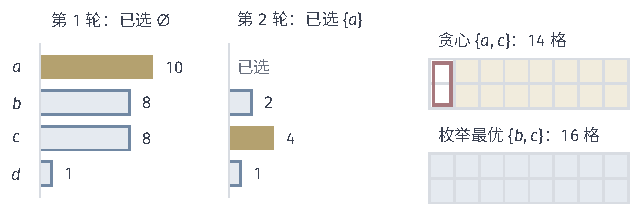
\includegraphics[width=107.177mm]{figures/01-basic-mathematics/04-graphs/tikz/c4-greedy-rounds-vs-optimum/figure.pdf}
  \caption{传感器实例上$k=2$的边际增益贪心。左侧两栏是两轮中各候选元素的当前增益，黄色条为该轮选中的元素；第$2$轮的增益相对于已选的$\{a\}$计算。右侧比较两个覆盖结果：贪心集合$\{a,c\}$（黄色）漏掉第$1$列两格（红框），枚举最优集合$\{b,c\}$（蓝色）覆盖全部$16$格。}
  \label{fig:graph-setfn-greedy-rounds}
\end{figure}

\subsection{算法分析}
\label{sec:graph-setfn-greedy-guarantee}

\paragraph{可行性}
算法每一轮恰好加入一个尚未选中的元素，执行$k$轮，所以输出恰有$k$个元素，满足基数约束；由于$k\leq n$，每一轮都有候选元素可选。$F$单调时每一轮的增益都非负，选满$k$个不会使目标下降。

\paragraph{近似保证}
实例中贪心的$14$与最优的$16$相差不多。这不是巧合，可以从“差距”的角度看清原因。记最优值与当前值之差为差距，第$1$轮开始时差距是$16-0=16$。

最优集合$O=\{b,c\}$只有两个元素，把它们加入当前集合能补上全部差距；它们相对于当前集合的增益分别是$8$和$8$，合计不少于差距，所以其中较大的一个至少补上差距的一半。贪心选的是全体元素中增益最大的，当然不比它差，实际选中的$a$补上了$10$。

第$2$轮开始时差距剩$6$，$b,c$相对于$\{a\}$的增益是$2$和$4$，合计仍不少于$6$，较大者至少是$3$，贪心选中的$c$补上$4$，差距降为$2$。图~\ref{fig:graph-setfn-greedy-gap-closing}画出这两轮比较。

\begin{figure}[!htb]
  \centering
  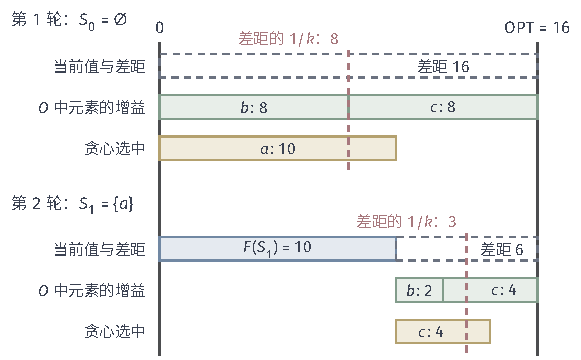
\includegraphics[width=98.446mm]{figures/01-basic-mathematics/04-graphs/tikz/c4-greedy-gap-closing/figure.pdf}
  \caption{贪心每轮至少补上差距的$1/k$（传感器实例，$k=2$，最优集合$O=\{b,c\}$）。每轮上行是当前值（蓝色）与到最优值$16$的差距（虚线框）；中行是$O$中元素相对于当前集合的增益（绿色），它们首尾相接至少覆盖整个差距；红色虚线标出差距的$1/k$，$O$中至少有一个元素的增益越过它；下行是贪心选中元素的增益（黄色），它不小于$O$中任何元素的增益。}
  \label{fig:graph-setfn-greedy-gap-closing}
\end{figure}

一般情形的论证与此相同。最优集合至多有$k$个元素，它们合起来能补上全部差距；由次模性，每个元素相对于当前集合的增益不小于它在“合起来补”时的那一份，所以这些增益之和不少于差距，其中最大者至少是差距的$1/k$。

贪心每轮至少补上剩余差距的$1/k$，差距每轮至多保留原来的$1-1/k$，经过$k$轮至多剩下$(1-1/k)^k$，不超过$e^{-1}$。这就像每期至少偿还剩余欠款的$1/k$，欠款按几何级数下降。

\begin{theorem}[贪心的近似保证]
\label{thm:graph-setfn-greedy-guarantee}
设$F$是有限底集$V$上的集合函数，满足$F(\varnothing)=0$、单调非减且次模；整数$1\leq k\leq|V|$。记$\mathrm{OPT}$为问题~\eqref{eq:graph-setfn-cardinality-problem}的最优值，$S_\ell$为算法~\ref{alg:graph-setfn-greedy}执行$\ell$轮后的集合（$0\leq\ell\leq k$）。则
\begin{equation}
  F(S_\ell)\geq\Bigl(1-\bigl(1-\tfrac1k\bigr)^{\ell}\Bigr)\mathrm{OPT}.
  \label{eq:graph-setfn-greedy-bound}
\end{equation}
特别地，
\[
  F(S_k)\geq\bigl(1-(1-1/k)^k\bigr)\mathrm{OPT}\geq(1-e^{-1})\mathrm{OPT}.
\]
\end{theorem}

\begin{proof}
固定一个最优集合$O$，$|O|\leq k$，$F(O)=\mathrm{OPT}$。考察第$t$轮开始时的集合$S_{t-1}$（$1\leq t\leq k$），先用次模性把它与最优值的差距上界为若干个边际增益之和。把$O\setminus S_{t-1}$中的元素排成$o_1,\ldots,o_r$，由单调性和式~\eqref{eq:graph-setfn-telescoping}，
\[
  \begin{aligned}
  \mathrm{OPT}=F(O)&\leq F(O\cup S_{t-1})\\
  &=F(S_{t-1})+\sum_{j=1}^{r}\Delta\bigl(o_j\mid S_{t-1}\cup\{o_1,\ldots,o_{j-1}\}\bigr).
  \end{aligned}
\]
每个$o_j$都不在$S_{t-1}\cup\{o_1,\ldots,o_{j-1}\}$中，由式~\eqref{eq:graph-setfn-diminishing-returns}，第$j$项满足
\[
  \Delta\bigl(o_j\mid S_{t-1}\cup\{o_1,\ldots,o_{j-1}\}\bigr)\leq\Delta(o_j\mid S_{t-1}).
\]
而贪心在第$t$轮选的是增益最大的元素，所以
\[
  \Delta(o_j\mid S_{t-1})\leq\Delta(v_t\mid S_{t-1})=F(S_t)-F(S_{t-1}).
\]
又$r\leq|O|\leq k$，且每一项增益非负，于是
\[
  \mathrm{OPT}-F(S_{t-1})\leq k\bigl(F(S_t)-F(S_{t-1})\bigr).
\]
也就是说，最优集合的至多$k$个元素合起来能补上的差距，至少有$1/k$能被当前最好的单个元素补上。

记差距$\delta_t=\mathrm{OPT}-F(S_t)$。上式可写成
\[
  \delta_{t-1}\leq k(\delta_{t-1}-\delta_t),
\]
即
\[
  \delta_t\leq\Bigl(1-\frac1k\Bigr)\delta_{t-1},\qquad t=1,\ldots,k.
\]
由$F(\varnothing)=0$得$\delta_0=\mathrm{OPT}$，连续使用$\ell$次得
\[
  \delta_\ell\leq(1-1/k)^\ell\,\mathrm{OPT},
\]
移项即为所求。

最后比较$(1-1/k)^k$与$e^{-1}$。函数$\psi(x)=e^{-x}-(1-x)$满足$\psi(0)=0$，导数$\psi'(x)=1-e^{-x}$在$x>0$时为正，所以$\psi$在$[0,+\infty)$上单调递增：闭区间上连续、内部导数为正的函数严格递增，这是微分中值定理的推论（可参考\BookChapterRef{chap:univariate-differentiation}{卷一“一元函数的微分”章}）。从而
\[
  0\leq1-x\leq e^{-x},\qquad 0\leq x\leq1.
\]
取$x=1/k$再求$k$次幂，得到
\[
  (1-1/k)^k\leq e^{-1}.
\]
\end{proof}

证明中三个条件各有作用。归一化保证差距从$\mathrm{OPT}$开始；若$F(\varnothing)\neq0$，给$F$加上一个常数会改变$F(S_k)$与$\mathrm{OPT}$的比值，比例式就失去意义。单调性用在$F(O)\leq F(O\cup S_{t-1})$和增益非负两处，次模性用在把$O$中元素的增益统一换成相对于$S_{t-1}$的增益。

$k=1$时界为$1$，贪心选出的就是最好的单元素；$k=2$时界为$3/4$。在传感器实例中逐轮核对定理给出的下界：
\[
  \begin{aligned}
  \ell=1:&\quad \tfrac12\times16=8\leq F(S_1)=10,\\
  \ell=2:&\quad \tfrac34\times16=12\leq F(S_2)=14,
  \end{aligned}
\]
两轮都与定理一致。

$1-e^{-1}\approx0.632$是对一切$k$都成立的比例，但它只是近似保证，贪心并不保证精确最优。

\paragraph{复杂度}
第$t$轮要对$n-t+1$个未选元素各求值一次，总共
\[
  \sum_{t=1}^{k}(n-t+1)\leq nk
\]
次求值，再加上开始时的一次$F(\varnothing)$。传感器实例$n=4$、$k=2$，共$1+4+3=8$次。若一次求值的代价为$\tau$（例如覆盖量需要合并若干覆盖范围），总代价是$O(nk\tau)$，选最大值等其余操作只占$O(nk)$。与枚举相比，$nk$次求值随$n,k$多项式增长，而可行子集的个数随$k$迅速增长。

\paragraph{适用范围}
撤去次模性，保证就不再成立。图~\ref{fig:graph-setfn-property-counterexamples}(a)的函数
\[
  F(S)=\max\bigl\{3\,\mathbb I\{\{1,2\}\subseteq S\},\ \mathbb I\{3\in S\}\bigr\}
\]
单调、归一化，但不是次模的。取$k=2$：第$1$轮三个增益依次为$0,0,1$，选$3$；第$2$轮相对于$\{3\}$，加入$1$或$2$的增益都是$0$，按编号选$1$，得到$F(\{1,3\})=1$。最优集合是$\{1,2\}$，$\mathrm{OPT}=3$。

元素$1,2$只有同时选中才有价值，每一轮单独看它们的增益都是零，贪心永远看不到这个互补组合。对照上面的差距论证，这里$O=\{1,2\}$合起来能补上差距$3$，各自的增益却都是$0$，“各元素增益之和不少于差距”这一步失效。把$3$换成任意大的$M$，比例$1/M$可以任意小，所以没有次模性就没有固定比例的保证。

撤去单调性同样会造成损失。图~\ref{fig:graph-setfn-property-counterexamples}(b)的单边割权是次模的，但不单调。取$k=2$并按算法~\ref{alg:graph-setfn-greedy}强制选满：第$1$轮选$1$（增益$1$），第$2$轮只剩$2$，增益为$-1$，仍须加入，结果$\operatorname{cut}(\{1,2\})=0$，而至多选两个时的最优值是$1$。在增益为负时停止可以避免这个例子中的损失，但对一般的非单调次模函数，这样修改后的贪心仍没有定理~\ref{thm:graph-setfn-greedy-guarantee}那样的保证，需要另外的算法与分析，本节不展开。

所以定理~\ref{thm:graph-setfn-greedy-guarantee}只适用于在基数约束下最大化归一化、单调、次模的集合函数，在这一范围内，贪心用至多$nk+1$次求值换来比例保证。贪心规则本身对任何集合函数都能执行，但目标、约束或函数性质改变时，保证都需要重新论证；下一节的预算约束就是一例。

\subsection{惰性贪心}
\label{sec:graph-setfn-lazy-greedy}

\subsubsection{问题与思路}

普通贪心每轮都重算全部未选元素的增益，其中许多元素的旧增益已经远低于领先者，本轮不可能被选中。次模性提供了一个省力的办法：已选集合只会变大，由式~\eqref{eq:graph-setfn-diminishing-returns}，元素的增益只会变小，所以早先算出的增益是它当前增益的上界。若某个元素刚刚重算出的增益不小于其他所有元素的旧增益，它就不小于这些元素的当前增益，可以直接选中，其余元素不必重算。

在实例的第$2$轮，三个候选的旧增益是$b{:}8$、$c{:}8$、$d{:}1$。先重算$b$，得$2$，它不再领先；再重算$c$，得$4$，不小于$b$的新值$2$与$d$的旧值$1$。$d$的当前增益不会超过$1$，不必重算，选$c$。这一轮只做了$2$次求值，选择与普通贪心相同。按这种方式缓存旧增益、只在必要时重算的实现称为\term{惰性贪心}（lazy greedy）。

\subsubsection{算法实现}

\paragraph{缓存增益的优先队列}
每轮都要找出缓存增益最大的元素，并在某个元素的增益重算后把它放回合适的位置，这由以缓存增益为键的最大优先队列完成。每个未选元素$v$在队列中恰有一个条目$(v,g_v,r_v)$：$g_v$是缓存的增益，$r_v$是算出它的轮次，即$g_v=\Delta(v\mid S_{r_v-1})$。轮次$r_v$用来判断缓存是否过期：$r_v$等于当前轮次时，$g_v$就是相对于当前集合的增益。

键的次序按$g_v$从大到小，$g_v$相同时编号小者在前，与普通贪心的平局规则一致。用到的操作只有两个：取出最前的条目，以及插入一个条目。用二叉堆实现时，两者都需要$O(\log n)$次比较。

\paragraph{惰性贪心的实现}
与算法~\ref{alg:graph-setfn-greedy}相同，底集、$k$和求值规则在运行前给定；此外要求$F$是次模的，否则旧增益不是上界，下面的选择可能与普通贪心不同。算法维护四项状态：
\begin{itemize}
  \item 已选集合$S$：初值为空集；
  \item 当前值$F(S)$：初值为一次求值得到的$F(\varnothing)$；
  \item 当前轮次$t$：正在进行的轮次，初值为$1$；
  \item 优先队列：每个未选元素一个条目$(v,g_v,r_v)$，初值$g_v=\Delta(v\mid\varnothing)$、$r_v=1$，由$n$次求值得到。
\end{itemize}
初始化共需$1+n$次求值，第$1$轮的缓存因此全部是新的。每一步取出队列最前的条目$(u,g_u,r_u)$，按两种情形处理：
\begin{itemize}
  \item 若$r_u=t$，缓存是新的：选中$u$，令$S\gets S\cup\{u\}$，$F(S)\gets F(S)+g_u$，$t\gets t+1$；
  \item 若$r_u<t$，缓存已过期：求值一次，令$g_u\gets\Delta(u\mid S)$、$r_u\gets t$，把条目放回队列。
\end{itemize}
$|S|=k$时停止，输出$S$。

\begin{algorithm}[惰性贪心]
\label{alg:graph-setfn-lazy-greedy}
输入：有限底集$V$（元素已编号），整数$0\leq k\leq|V|$，单调非减且次模的集合函数$F$的求值规则。输出：与算法~\ref{alg:graph-setfn-greedy}相同的集合。
\begin{enumerate}
  \item 令$S=\varnothing$，记录$F(\varnothing)$，$t=1$；对每个$v\in V$求$g_v=\Delta(v\mid\varnothing)$，令$r_v=1$，把$(v,g_v,r_v)$插入队列。
  \item 当$|S|<k$时，取出队列最前的条目$(u,g_u,r_u)$。
  \item 若$r_u=t$，令$S\gets S\cup\{u\}$，$F(S)\gets F(S)+g_u$，$t\gets t+1$；否则求$g_u=\Delta(u\mid S)$，令$r_u=t$，把条目放回队列。回到第2步。
  \item 输出$S$。
\end{enumerate}
\end{algorithm}

\paragraph{执行过程}
为了看到旧缓存跨越两轮的情形，在传感器实例上取$k=3$。初始化求值$F(\varnothing)=0$与四个单元素增益，队列为$a{:}10$、$b{:}8$、$c{:}8$、$d{:}1$，轮次都是$1$。表~\ref{tab:graph-setfn-lazy-trace}逐步列出取出的条目、所做的处理和处理后的队列。
\begin{itemize}
  \item 第$1$轮：取出$a$，缓存是新的，直接选中，$S=\{a\}$，$F=10$。
  \item 第$2$轮：取出$b$，缓存来自第$1$轮，重算得$2$后放回；取出$c$，重算得$4$后放回，排到最前；再取出$c$，缓存是新的，选中，$S=\{a,c\}$，$F=14$。$d$的旧值$1$始终排在后面，没有重算。
  \item 第$3$轮：取出$b$，它的缓存$2$来自第$2$轮，已过期，重算仍得$2$后放回；再取出$b$，选中，$S=\{a,b,c\}$，$F=16$。
\end{itemize}
此时$|S|=3$，停止。三轮的选择与普通贪心逐轮重算的结果一致，求值共$1+4+2+1=8$次，普通贪心需要$1+4+3+2=10$次。

\begin{table}[!htb]
  \centering
  \caption{传感器实例上$k=3$的惰性贪心。每行是一次取出：“重算”表示缓存过期而求值一次后放回，“选中”表示缓存是新的；队列按键的次序列出，每项写元素、缓存增益与算出它的轮次。}
  \label{tab:graph-setfn-lazy-trace}
  \small
  \begin{tabular}{@{}cccl@{}}
    \toprule
    轮 & 取出 & 处理 & 处理后的队列 \\
    \midrule
    初始 & — & 求值$5$次 & $a(10,1)$，$b(8,1)$，$c(8,1)$，$d(1,1)$ \\
    $1$ & $a(10,1)$ & 选中 & $b(8,1)$，$c(8,1)$，$d(1,1)$ \\
    $2$ & $b(8,1)$ & 重算得$2$ & $c(8,1)$，$b(2,2)$，$d(1,1)$ \\
    $2$ & $c(8,1)$ & 重算得$4$ & $c(4,2)$，$b(2,2)$，$d(1,1)$ \\
    $2$ & $c(4,2)$ & 选中 & $b(2,2)$，$d(1,1)$ \\
    $3$ & $b(2,2)$ & 重算得$2$ & $b(2,3)$，$d(1,1)$ \\
    $3$ & $b(2,3)$ & 选中 & $d(1,1)$ \\
    \bottomrule
  \end{tabular}
\end{table}

\subsubsection{算法分析}

\paragraph{正确性}
惰性贪心每轮选出的元素与普通贪心按同一平局规则选出的相同，从而定理~\ref{thm:graph-setfn-greedy-guarantee}的保证原样适用。证明对轮次归纳：设前$t-1$轮两者选出相同元素，当前集合都是$S_{t-1}$。

在第$t$轮，设取出的条目$(u,g_u,t)$缓存是新的，则$g_u=\Delta(u\mid S_{t-1})$。对队列中任一其他元素$v$，它的缓存$g_v=\Delta(v\mid S_{r_v-1})$是在更小的集合$S_{r_v-1}\subseteq S_{t-1}$上算出的，由式~\eqref{eq:graph-setfn-diminishing-returns}，
\[
  g_v\geq\Delta(v\mid S_{t-1}).
\]
$u$排在$v$前面，所以
\[
  \Delta(u\mid S_{t-1})=g_u\geq g_v\geq\Delta(v\mid S_{t-1}).
\]
若某个$v$的当前增益与$u$相等，则$g_v$也与$g_u$相等，$u$排在前面说明它的编号更小。所以$u$正是普通贪心第$t$轮的选择。

每一轮都会结束：每次重算都把一个过期条目变成新的，一轮内至多重算$n-t+1$次，之后队列最前的条目必定是新的而被选中。

这里的正确性只用到次模性，没有用到单调性和归一化；它们是近似保证需要的条件。对一般函数，旧增益不是上界，排在后面的元素的当前增益可能已经超过选中的元素，因此必须每轮全部重算。

\paragraph{复杂度}
初始化需要$1+n$次求值。第$t\geq2$轮的重算次数不超过未选元素个数$n-t+1$，所以最坏情形的求值次数与普通贪心相同；省下多少取决于增益下降的快慢，没有一般的保证。

每次重算伴随一次取出与一次插入，每轮再有一次取出用于选中，每次队列操作需要$O(\log n)$次比较，最坏总开销为$O(nk\log n)$次比较，另加初始插入的$O(n\log n)$次比较。队列存放$n$个条目，额外空间为$O(n)$。一次求值的代价$\tau$通常远大于$O(\log n)$，这时省下的求值次数决定了实际运行时间。

% 第9章第2节：预算约束下的子集选择（问题与思路；算法实现；算法分析）。

\section{预算约束下的子集选择}
\label{sec:graph-budget-selection}

基数约束让每个元素占用一个名额。实际中不同传感器的价格不同，限制的往往是总花费而不是个数。逐轮贪心仍然可用，但比较的对象要改成单位成本的增益。本节说明这一改动的理由与实现，再用反例说明上一节的近似保证不能直接搬到预算约束下。

\subsection{问题与思路}
\label{sec:graph-setfn-budget-problem}

给每个元素$v\in V$指定成本$c_v$，再给定总预算$B\geq0$。要求的是
\begin{equation}
  \max_{S\subseteq V}\ F(S)\qquad\text{满足}\quad\sum_{v\in S}c_v\leq B.
  \label{eq:graph-setfn-budget-problem}
\end{equation}
满足成本条件的子集称为预算可行的，这一条件称为\term{预算约束}（budget constraint）。目标函数$F$与上一节相同，改变的只是允许的子集。所有成本都取$1$、预算取$k$时，预算约束就是基数约束，所以本节的问题是上一节的推广。

成本为零的元素需要先单独处理。零成本元素不占预算，若$F$单调，把它们全部加入不会降低目标，可以在开始时一次放进集合；若$F$不单调，它们是否值得加入要看增益的正负。以下设所有成本为正。另外，成本超过$B$的元素不可能出现在任何可行集合中，可以预先删去。

下面在传感器实例上取第~\ref{sec:graph-setfn-definition}小节的成本，并给定预算：
\[
  c_a=4,\quad c_b=3,\quad c_c=4,\quad c_d=1,\qquad B=7.
\]
预算可行的子集共有$10$个：空集、四个单元素集，以及$\{a,b\}$（成本$7$）、$\{a,d\}$（$5$）、$\{b,c\}$（$7$）、$\{b,d\}$（$4$）、$\{c,d\}$（$5$）；三元及以上的子集成本都超过$7$。枚举得最优集合为$\{b,c\}$，覆盖$16$格。

与$k=2$的基数约束相比，$\{a,c\}$成本为$8$，现在不可行了；而$\{a,b\}$在两种约束下都可行。选择的个数不再直接决定资源消耗，每次加入元素前都要检查剩余预算。

把上一节的贪心原样搬过来，就是每轮在付得起的元素里选增益最大的。这样做可能偏爱昂贵的元素：一个元素增益大，可能只是因为它贵，而它占去的预算本可以换来更多增益。预算是按成本消耗的，所以更合理的比较是每单位成本带来多少增益，即比值$\Delta(v\mid S)/c_v$。

这样得到单位成本规则：每轮选比值最大且付得起的元素，直到剩余预算放不下任何元素，或者付得起的元素都不再带来增益。

\subsection{算法实现}
\label{sec:graph-setfn-ratio-greedy}

成本$c_v$、预算$B$和求值规则在运行前给定，运行中不变，不算状态。与上一节相比，算法多记录剩余预算，并且每轮只在付得起的元素中比较。算法维护四项状态：
\begin{itemize}
  \item 已选集合$S$：初值为空集；
  \item 剩余预算$R=B-\sum_{v\in S}c_v$：初值为$B$；
  \item 当前值$F(S)$：初值由一次求值得到$F(\varnothing)$，此后每轮加上选中元素的增益；
  \item 本轮增益：每个付得起的未选元素$v$相对于当前$S$的增益$\Delta(v\mid S)$，每轮重新计算。
\end{itemize}
初始化令$S=\varnothing$、$R=B$，并求值一次得到$F(\varnothing)$。每一轮做四件事：
\begin{itemize}
  \item 列候选：记$Q=\{v\in V\setminus S:c_v\leq R\}$为付得起的未选元素；若$Q$为空，停止；
  \item 求增益：对每个$v\in Q$求值，得到$\Delta(v\mid S)$；若这些增益全为零，停止；
  \item 选择：取比值$\Delta(v\mid S)/c_v$最大的$v$，比值相同时取编号最小者；
  \item 更新：令$F(S)\gets F(S)+\Delta(v\mid S)$，再令$S\gets S\cup\{v\}$，$R\gets R-c_v$。
\end{itemize}
停止条件因此有两个：剩余预算放不下任何未选元素，或者付得起的元素都不再增加目标。

\begin{algorithm}[预算约束下的单位成本贪心]
\label{alg:graph-setfn-ratio-greedy}
输入：有限底集$V$（元素已编号），正成本$c_v$，预算$B\geq0$，单调非减集合函数$F$的求值规则。输出：预算可行的集合。
\begin{enumerate}
  \item 令$S=\varnothing$，$R=B$，记录$F(\varnothing)$。
  \item 记候选集合$Q=\{v\in V\setminus S:c_v\leq R\}$。若$Q$为空，停止。
  \item 对每个$v\in Q$计算$\Delta(v\mid S)$。若这些增益全为零，停止；否则取比值$\Delta(v\mid S)/c_v$最大的$v$，比值相同时取编号最小者。
  \item 令$S\leftarrow S\cup\{v\}$，$R\leftarrow R-c_v$，回到第2步。
\end{enumerate}
\end{algorithm}

\paragraph{执行过程}
在$B=7$的实例上，表~\ref{tab:graph-setfn-ratio-trace}逐轮记录状态。
\begin{itemize}
  \item 第$1$轮：$R=7$，四个元素都付得起，增益是各自的覆盖量，比值依次为
  \[
    a{:}\ 10/4=2.5,\quad b{:}\ 8/3\approx2.67,\quad c{:}\ 8/4=2,\quad d{:}\ 1/1=1.
  \]
  选$b$，$R=4$。
  \item 第$2$轮：$Q=\{a,c,d\}$，增益相对于$\{b\}$重新计算。$a$只补上第$5$、$6$列的$4$格，比值$1$；$c$与$b$不重叠，增益$8$，比值$2$；$d$那一格已被$b$覆盖，增益$0$。选$c$，$R=0$。
  \item 第$3$轮：没有成本不超过$0$的元素，$Q$为空，停止。
\end{itemize}
输出$\{b,c\}$，覆盖$16$格，恰为枚举最优值。

\begin{table}[!htb]
  \centering
  \caption{$B=7$时单位成本贪心的状态表（成本$c_a=4$、$c_b=3$、$c_c=4$、$c_d=1$）。每格写增益，括号内为增益与成本之比；“—”表示已选或付不起；最后一列是本轮选中的元素与更新后的剩余预算。}
  \label{tab:graph-setfn-ratio-trace}
  \small
  \begin{tabular}{@{}cccccccc@{}}
    \toprule
    轮 & $S$ & $R$ & $a$ & $b$ & $c$ & $d$ & 选中，新$R$ \\
    \midrule
    $1$ & $\varnothing$ & $7$ & $10\ (2.5)$ & $8\ (2.67)$ & $8\ (2)$ & $1\ (1)$ & $b$，$4$ \\
    $2$ & $\{b\}$ & $4$ & $4\ (1)$ & — & $8\ (2)$ & $0\ (0)$ & $c$，$0$ \\
    $3$ & $\{b,c\}$ & $0$ & — & — & — & — & $Q$为空，停止 \\
    \bottomrule
  \end{tabular}
\end{table}

作为对照，按总增益最大选择的规则在第$1$轮选$a$（增益$10$），剩余预算$3$；第$2$轮付得起的有$b$（增益$2$）和$d$（增益$1$），$c$的成本$4$超出剩余预算，选$b$，剩余预算$0$，停止，覆盖$12$格。图~\ref{fig:graph-setfn-budget-rule-comparison}把两种规则的选择画在同一条预算上：昂贵的$a$一开始就占去一半以上的预算，之后只剩小元素可选。

\begin{figure}[!htb]
  \centering
  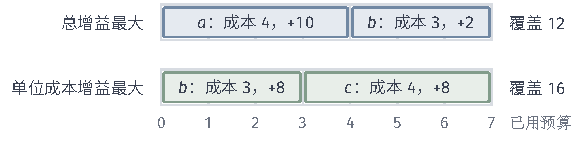
\includegraphics[width=98.538mm]{figures/01-basic-mathematics/04-graphs/tikz/c4-budget-rule-comparison/figure.pdf}
  \caption{预算$B=7$下两种逐轮规则的选择结果（成本$c_a=4$、$c_b=3$、$c_c=4$、$c_d=1$）。每条横条代表$7$个单位的预算，色块的宽度是所选元素的成本，块内写出选择时的增益。按总增益先选昂贵的$a$，剩余预算只够再选增益$2$的$b$，覆盖$12$格；按单位成本先选$b$，再选$c$，覆盖$16$格。}
  \label{fig:graph-setfn-budget-rule-comparison}
\end{figure}

\paragraph{最佳单元素比较}
单位成本规则也有自己的偏差：它可能先选几个便宜的小元素，把预算切碎，使一个昂贵但价值很高的元素再也放不进去。

一种简单的补救是在算法结束后增加一步：计算每个可行单元素的值$F(\{v\})$（$c_v\leq B$），输出$S$与最佳单元素中函数值较大的一个。这只需另外$n$次求值。

在$B=7$的实例中，最佳单元素是$\{a\}$，覆盖$10$格，小于$16$，输出仍是$\{b,c\}$。这一检查只是一个具体策略；本节没有给出它的分析，因此不附加任何近似比例。

\subsection{算法分析}
\label{sec:graph-setfn-budget-limits}

\paragraph{可行性}
算法始终保持$R=B-\sum_{v\in S}c_v\geq0$：初始时$R=B\geq0$；每轮只从$Q$中选元素，而$Q$中元素的成本不超过$R$，减去后$R$仍非负。所以输出总是预算可行的。

\paragraph{停止性}
每轮加入一个新元素，至多执行$n$轮就会停止。停止时有两种原因：没有付得起的元素，或者付得起的元素都不再增加目标。

对单调函数，后一种情形下再加入任何一个付得起的元素都不会提高函数值；若函数还是次模的，按上一节提前停止的论证，一次加入若干个付得起的元素也不会提高函数值。

\paragraph{复杂度}
第$t$轮的候选元素不超过$n-t+1$个，所以求值次数不超过
\[
  n+(n-1)+\cdots+1=\frac{n(n+1)}{2},
\]
再加开始时的一次$F(\varnothing)$；附加最佳单元素比较时另加$n$次。上面的实例做了$1+4+3=8$次求值。若一次求值的代价为$\tau$，总代价为$O(n^2\tau)$。

\paragraph{适用范围}
单位成本规则在上面的实例中表现很好，但它本身没有任何固定比例的保证。

\begin{example}[比值规则的失效]
\label{ex:graph-setfn-ratio-failure}
底集$\{u,w\}$，预算$B=100$。$u$的成本为$1$、价值为$2$，$w$的成本为$100$、价值为$100$，目标取模函数$F(S)=\sum_{v\in S}(\text{价值})$。各价值非负，所以它归一化、单调，也是次模的。

比值规则第$1$轮比较$2/1=2$与$100/100=1$，选$u$；剩余预算$99<100$，$w$付不起，算法停止，得$F(\{u\})=2$。最优选择是$\{w\}$，$F=100$。见图~\ref{fig:graph-setfn-budget-ratio-failure}。

把$w$的成本、价值与预算同时换成任意大的$M$，比值规则仍先选$u$，得到$2$而最优值为$M$，比例$2/M$可以任意小。
\end{example}

\begin{figure}[!htb]
  \centering
  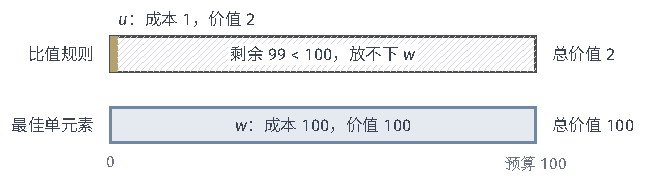
\includegraphics[width=109.146mm]{figures/01-basic-mathematics/04-graphs/tikz/c4-budget-ratio-failure/figure.pdf}
  \caption{比值规则的失效例。横条长度代表预算$100$。上行：比值规则先选单位价值较高的$u$（黄色，成本$1$，为便于观察略加宽），剩余$99$个单位（斜线）放不下成本$100$的$w$，总价值$2$。下行：最佳单元素$w$恰好用满预算，总价值$100$。}
  \label{fig:graph-setfn-budget-ratio-failure}
\end{figure}

这个例子的目标是模函数，从而归一化、单调且次模，满足上一节定理的全部函数条件。比值规则仍不能继承那里的保证，原因在于上一节差距论证的关键一步没有对应物。

那里最优集合的至多$k$个元素在每一轮都仍然可选，所以当前最好的元素至少补上差距的$1/k$。预算约束下，选进一个便宜元素就可能让最优集合中的元素再也付不起：例中选了$u$以后，差距是$100-2=98$，而最优集合唯一的元素$w$已经放不进剩余的$99$个单位，可选的元素一个也没有，差距一点也补不上。

最佳单元素比较能修复这个例子，但修复一个例子不构成一般保证；有严格保证的预算选择算法需要另外的枚举或修正机制及其证明，本书不展开。

\paragraph{结果检验}
小实例可以枚举全部预算可行子集，核对总成本、函数值以及与最优值的差距：$B=7$时比值规则的$\{b,c\}$与枚举最优一致，总增益规则的$\{a,b\}$差$4$格。

大实例无法枚举时，至少应报告剩余预算、最终目标值、最佳单元素的值和总求值次数；若逐轮规则的结果不如最佳单元素，往往就是出现了示例~\ref{ex:graph-setfn-ratio-failure}那样预算被小元素切碎的情形。

\paragraph{与基数约束贪心的比较}
两种贪心的状态与更新几乎相同，差别只在选择依据换成单位成本的增益，停止条件换成剩余预算放不下有增益的元素。所有成本都取$1$、预算取$k$时，单位成本规则除了增益全为零时提前停止以外，就是上一节的贪心。

对同样的归一化单调次模目标，基数约束下有$1-(1-1/k)^k$的保证，预算约束下简单的比值规则却可以任意差：约束的形式本身就决定算法能否得到保证。

\FloatBarrier
\section{本章小结}
\label{sec:subset-selection-chapter-summary}

本章回答了名额或经费有限时怎样选子集。两种贪心有相同的骨架：从空集出发，逐轮维护已选集合与当前值，相对于当前集合重算增益，加入一个元素。基数约束下比较的是边际增益本身，预算约束下比较的是单位成本的增益，并且只在付得起的元素中比较。两者都只需多项式次求值，分别至多$nk+1$次和$n(n+1)/2+1$次，总代价还要乘以每次求值的开销。

贪心规则本身对任何集合函数都能执行，但结果有没有保证取决于目标性质和约束。基数约束下最大化归一化、单调、次模的函数时，最优集合的至多$k$个元素在每一轮都仍然可选；由次模性，当前最好的元素至少补上剩余差距的$1/k$，差距按几何级数缩小，贪心值不低于最优值的$1-(1-1/k)^k$倍，从而不低于$1-e^{-1}$倍。撤去次模性，贪心看不到只有同时选中才有价值的互补组合；撤去单调性，强制选满会降低目标。两种情形下比例保证都不再成立。

惰性贪心是同一规则的另一种实现。次模性使旧增益成为当前增益的上界，优先队列据此只重算排在最前的元素；在一致的平局规则下，它与普通贪心逐轮选出相同的元素，所以继承同样的保证。它的正确性只需要次模性，节省多少求值没有一般的保证，最坏情形与普通贪心相同。

预算约束改变了可行性，也改变了分析。单位成本规则在传感器实例中找到最优解，却在成本与价值分别为$(1,2)$与$(100,100)$的例子中可以任意差：选进便宜元素以后，最优集合的元素可能再也放不进剩余预算，差距论证中“最优集合的元素仍可选”这一步失效。最佳单元素比较能修复这个例子，但本章没有证明它的一般比例。使用任何一种选择方法之前，都要写明目标方向、约束形式、函数是否归一化、单调和次模。

下一章转向最小化方向，没有基数或预算约束，但要求目标由一元项和成对项组成；在相应的次模条件下，最小割给出精确解。

